\documentclass[a4paper, 12pt,oneside]{article} 
%\documentclass[a4paper, 12pt,oneside,draft]{article} 
\usepackage{preamble}
\usepackage{pythonhighlight}

%--------------------- ACTUAL FILE ---------------------- %
\begin{document} 
%%%
	%\setcounter{page}{1}
	\begin{center}
	    \Large
	    \textbf{HMC : When is it worth over RWMC ?} 
	    \vspace{0.4cm}
	    \large

		Course : Stochastic Simulation \\
	    Students : Aude Maier \& Tara Fjellman \\
	    \small{Fall 2024}
	\end{center}

	\section{Introduction}
	\section{Core Theory}
		\subsection{RWMC}
		\subsection{HMC}
			\subsubsection{The Algorithm}
			\subsubsection{Acceptance Rate}
			\subsubsection{Convergence to Target Distribution}
			\paragraph{Gibbs distribution invariance}
			Under the assumption that there is no numerical error, we want to prove that the Gibbs measure is invariant for the chain generated by the hamiltonian dynamics.
	
			This is equivalent to saying that the Gibbs measure $\pi$ is the same before and after an evolution of $t$ seconds from the hamiltonian dynamics. 
			To prove this we first introduce hamiltonian dynamics operators $\phi,\Phi$ acting respectively on the phase space and the Gibbs measure : $\phi_t(q_s,p_s)=(q_{s+t},p_{s+t});\Phi_t[\pi_s]=\pi_{t+s}\quad \forall t\in\mathbb{R}$.
			The statement we want to prove can then be expressed as 
			\begin{gather}
				\Phi_t[\pi_s](D)=\pi_{s+t}(D)\quad \forall D\in\mathcal{B}(\Omega),\forall s,t\in\mathbb{R},
				%P(T_t(q,p)\in D_s)=
				%P((q,p)\in T_{-t}(D_s))=
				%P((q,p)\in D_s)=\pi(D_s),
				%P((q,p))=\int_{\Omega} K((q,p),D_s) G(q,p) \ dq dp=\pi(T_t[D_s]),
			\end{gather}
			with $\Omega$ the phase space.
	
			We can now write the left hand side of the equation as
			\begin{align}
				\Phi_t[\pi_s](D)&=\int_D \pi_{s+t}(q,p)\ dqdp \\
					&=\int_{\phi_{-t}(D)}\pi_{s}(q,p)\ dqdp \\
					&=\pi_s(\phi_{-t}(D)).
			\end{align}
			The final result is obtained using the fact that volumes in phase space are preserved by the hamiltonian dynamics (in conservative systems). This result is known as Liouville's theorem, but is mentioned as theorems 2.3 in [cite].
			%K:\Omega \times D\to [0,1]$ the transition kernel of the chain, $G(q,p)$ the Gibbs distribution, and $T_t[\cdot]$ the hamiltonian time evolution operator defined by $T[(q_s,p_s)]=(q_{s+t},p_{s+t})$.
	
			This implies specifically that $q_k\sim\pi$ for all $k\in\mathbb{N}$ if $q_0\sim \pi$. 
	
			If the dynamics is discretised with the Velocity Verlet algorithm, the volume in phase space is preserved up to a small error, which is why the algorithm is used in practice [cite wikipedia]. 
			\paragraph{What happens for discrete evolution ?}

	\section{Exploring a 2D example}
		\subsection{Context}
		In this section we explore the performance of the presented algorithms on a 2D example. The target distribution is taken as $f_1(q_1,q_2)=e^{-\alpha(q_1^2+q_2^2-0.25)^2}$, with $\alpha>0$ a parameter. This unormalised density is represented in figure \ref{fig:alpha-density} for two different values of $\alpha$.
        \begin{figure}[htb]
            \centering
                \vspace{0em}
                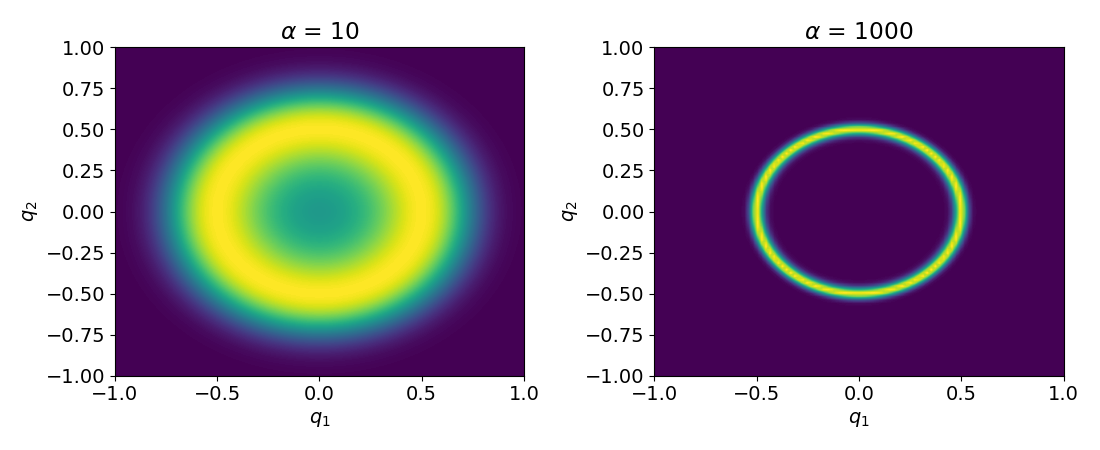
\includegraphics[width=0.9\textwidth]{alpha_density}
                \caption{Density considered in this section for two different values of $\alpha$.}
                \label{fig:alpha-density}
        \end{figure}
		As it can be seen, the density has the shape of a doughnot and $\alpha$ controls its thickness. We expect the $\alpha=1000$ case to be more difficult to sample from than the $\alpha=10$ case, as the density is more localised.
		\subsection{RWMC Solution}
			As seen previously, the RWMC algorithms only depends on the step size. To find the best RWMC sampler we therefore explore the impact of the step size on performance. 
			
			Here and in the following, We decide to quantify performance throught the computation of a similarity based on the Jensen-Shannon divergence. This choice allows us to feed in a discretised version of $f_1$ (which we can normalise) and the empirical distribution of the samples generated by the algorithm, and get a similarity measure between the two.

			The similarities associated to 3000 samples for the different step sizes are presented in figure \ref{fig:rwmc-scan}.
			\begin{figure}[htb]
				\centering
					\vspace{0em}
					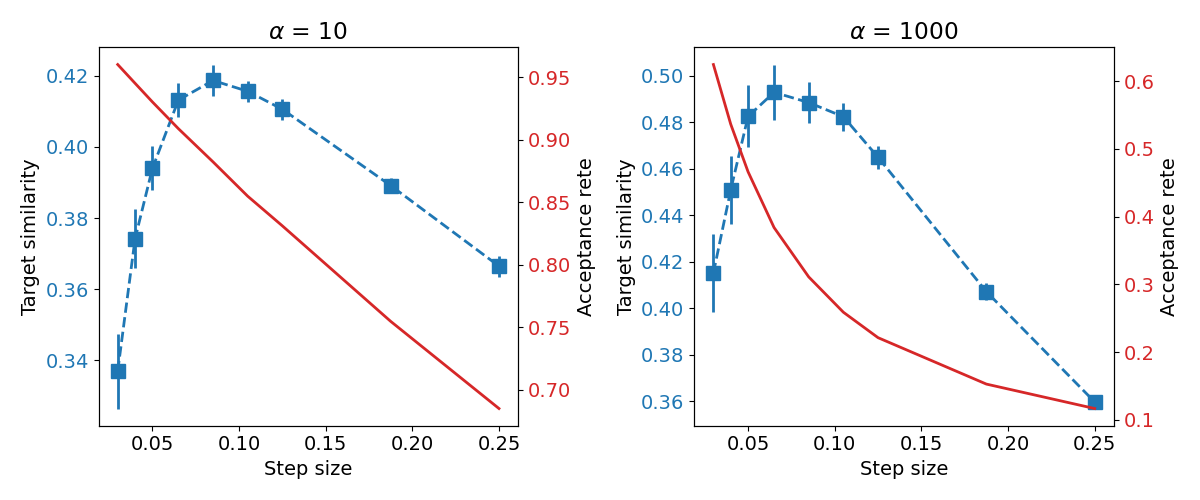
\includegraphics[width=0.95\textwidth]{rwmc_scan}
					\caption{Similarity as a function of RWMC step size for considered values of $\alpha$.}
					\label{fig:rwmc-scan}
			\end{figure}

			- both plots display a peak for a step size in the centre of the range considered (around 8.5$\times 10^{-2}$ and 6.5$\times 10^{-2}$ for $\alpha=10$ and $\alpha=1000$ respectively). This is expected as the step size is a tuning parameter that should be chosen to match the scale of the target distribution.
			- the peak is sharper (espescially on the right) for the $\alpha=1000$ case, which is consistent with the fact that the density is more localised. 
			- the value of the similarity is in all cases smaller than .5, which means that 3000 samples are too few to accurately estimate the target distribution. The value is higher in the $\alpha=1000$ case, which can at first look surprising. Indeed, this case is meant to be harder than the $\alpha=10$ one, but the fact that the density is more localised for $\alpha=1000$ actually means that there are fewer places where the estimate and the target can differ, which can lead to a better similarity. It is therefore most important to consider the relative values of the similarities for the different step sizes, rather than the absolute values.
			- looking at acceptance rate, we see that they are of course monotonically deacreasing with step size. This means that the obtimal value corresponds with the best exploration-acceptance rate trade-off. The acceptance rate is higher and decreases slower for the $\alpha=10$ case, which is consistent with the fact that the density is more spread out. The acceptance rate of the $\alpha=1000$ case associated to the best step size is still around .55, which suggests that this case is still quite easy to sample from. 
		\subsection{HMC Solution}
			\begin{wrapfigure}[18]{r}{0.6\textwidth}
				\centering
					\vspace{-2em}
					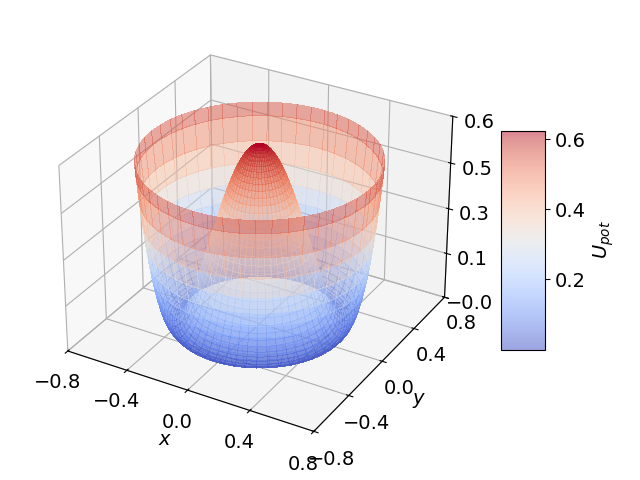
\includegraphics[width=0.57\textwidth]{U_pot_alpha=10}
					\caption{Potential energy landscape associated to HMC algorithm for $\alpha=10$. Version for $\alpha=1000$ is identical, except scales are scaled by a factor of 100.}
					\label{fig:U-pot-alpha=10}
			\end{wrapfigure}
			Before exploring the impact of the different parameters of the HMC algorithm, we first present the potential energy landscape associated to the algorithm for this specific problem. The landscape is presented in figure \ref{fig:U-pot-alpha=10}. 
			The landscape has polar symmetry, meaning the trajectories will be circles of fixed radius. It has global minima at a radius of 0.5 [CHECK] away from the centre and a local maxima at the centre. The only difference in the landscape for $\alpha=1000$ w.r.t. the $\alpha=10$ one is the scale of the potential. This means that the $\alpha=1000$ will give rise to stronger potential forces, which translates the fact that the density is more localised. 
			\subsubsection{Impact of Integration Time}
			The first parameter we explore is the integration time. For this parameter, we expect the optimal value to be the one that allows the sampler to explore the whole space, without being excessively long (as it would slow down sampling).
			The similarities associated to 3000 samples for the different integration times are presented in figure \ref{fig:t-scan}.

			- qualitatively same behaviour : increase of similarity with integration time, followed by a plateau (though more noisy for $\alpha=1000$ case).
			- the plateau is reached quicker for the $\alpha=10$ case, probably because the forces are stronger and the sampler can explore the space more quickly.
			- good values for the integration time 
			\begin{figure}[htb]
				\centering
					\vspace{0em}
					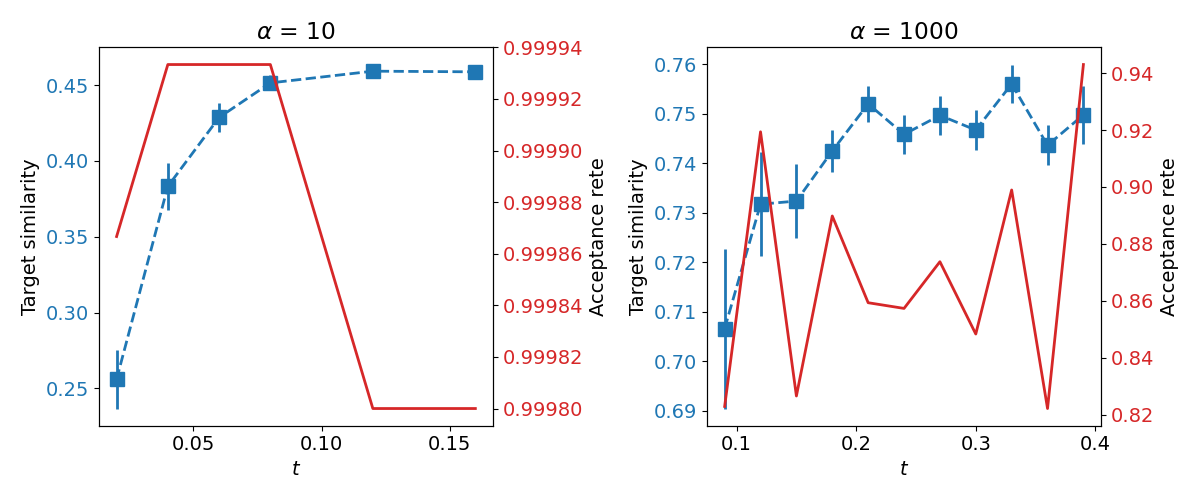
\includegraphics[width=0.95\textwidth]{t_scan}
					\caption{Similarity as a function of HMC integration time for considered values of $\alpha$.}
					\label{fig:t-scan}
			\end{figure}
			\lipsum[1]
			\subsection{Impact of $\Delta t$}
			\begin{figure}[htb]
				\centering
					\vspace{0em}
					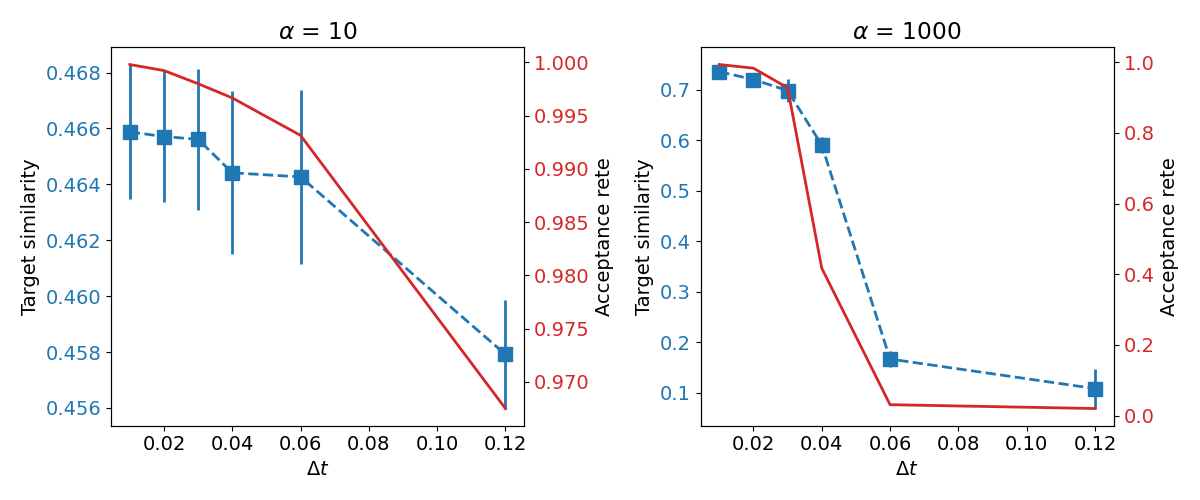
\includegraphics[width=0.95\textwidth]{dt_scan}
					\caption{Similarity as a function of HMC time step for considered values of $\alpha$.}
					\label{fig:dt-scan}
			\end{figure}
			\lipsum[1]
			\subsection{Impact of Mass Scale}
			\begin{figure}[htb]
				\centering
					\vspace{0em}
					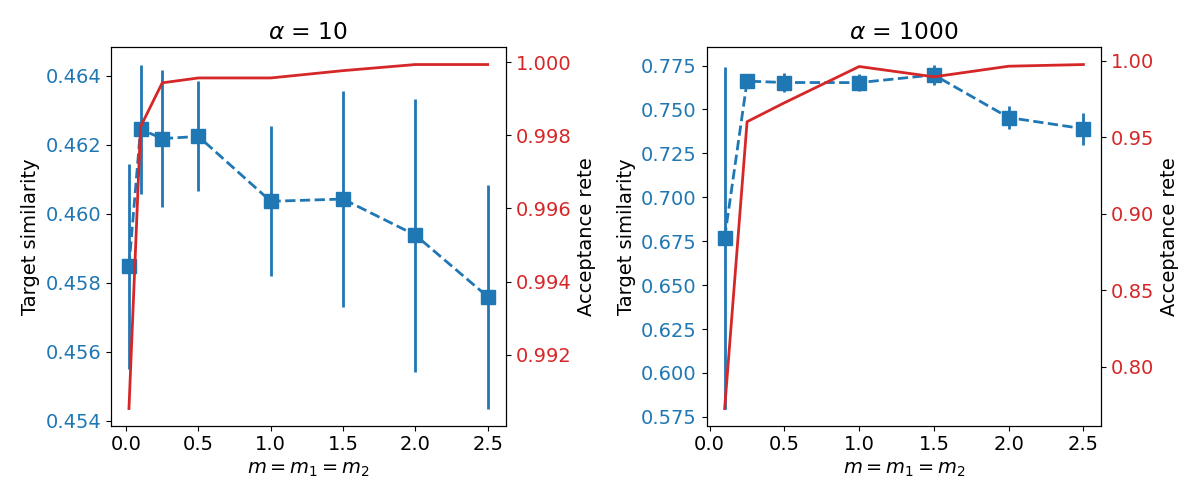
\includegraphics[width=0.95\textwidth]{mass_scan}
					\caption{Similarity as a function of HMC mass scale for considered values of $\alpha$.}
					\label{fig:mass-scan}
			\end{figure}
			\lipsum[1]
			\subsection{Impact of Mass Symmetry}
			\begin{figure}[htb]
				\centering
					\vspace{0em}
					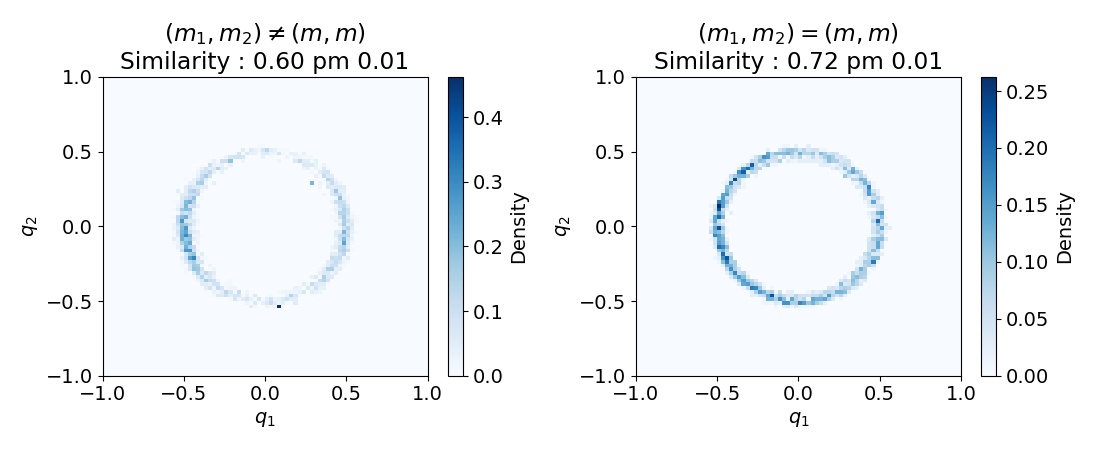
\includegraphics[width=0.95\textwidth]{mass_sym}
					\caption{Similarity for HMC samplers with asymmetric and symmetric masses for $\alpha=1000$.}
					\label{fig:mass-sym}
			\end{figure}
			\lipsum[1]
		\subsection{Comparison and Sample-Size Evolution}
		\begin{figure}[htb]
			\centering
				\vspace{0em}
				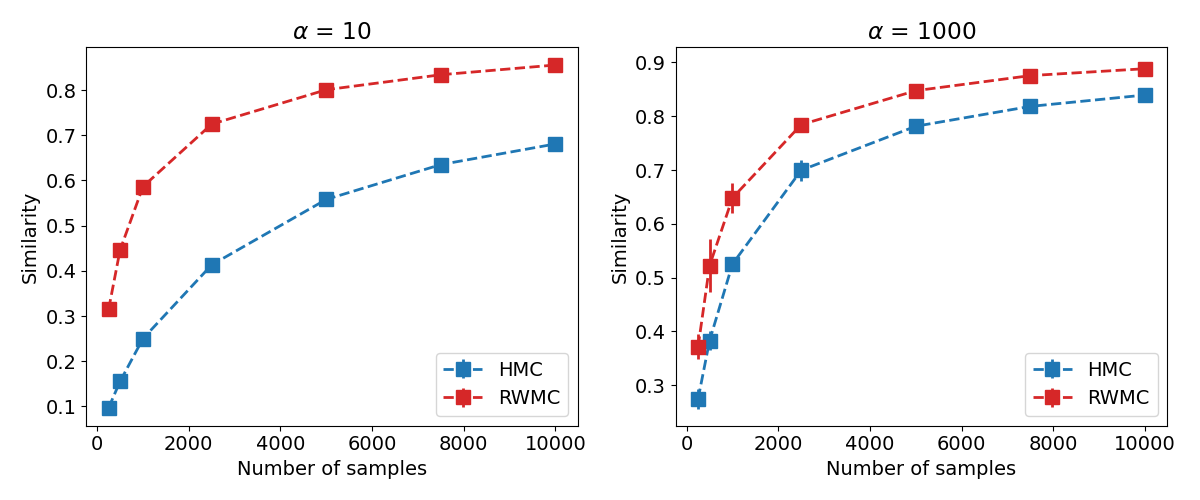
\includegraphics[width=0.9\textwidth]{nsamples_evolution}
				\caption{Similarity as a function of sample-size for RWMC and HMC samplers and considered values of $\alpha$. The sample-size represented on the x axis is that associated to the HMC sampler. The associated RWMC sample-size is obtained by matching the number of function evalutations of the HMC sampler.}
				\label{fig:nsamples-evolution}
		\end{figure}
		\lipsum[1]
	\section{US Birthweight Data}
		\subsection{HMC Solution}
		\subsection{RWMC Solution}
	\section{(f)}
	\section{Section ...}
	\section{Conclusion}
	\section*{Aknowledgements}
	\section*{References}
	\appendix
		\section{Commented Code Snippet}\label{appendix:commented-code-snippet}
			[cite stack exchange for format]
			\begin{python}
			if transactions: Transaction.create_transactions() # if transactions = "true"
			node.generate_emptyState() # empty state for all nodes
			S.initial_events() # initiate initial events to start with

			while not queue.isEmpty() and clock <= targetTime:
				next_e = queue.get_next_event()
				clock = next_e.time # move clock to the time of the event
				Event.execute_event(next_e)
				Queue.remove_event(next_e)

			print results
			\end{python}
		\section{Rejection Sampling Attempt}\label{appendix:rejection-sampling-attempt}
		As an alternative to HMC we consider rejection sampling. We therefore want to find a function $g(q)$ and a constant $C$ such that the following inequality holds for all $q$:
		\begin{equation}
			\tilde{f}(q) = e^{q^TX^T(y-1_{n})}e^{-1_{n}^T \log[1+\exp(-x_i^Tq)]_{n\times 1}}e^{-\frac{1}{2}q^T\Sigma^{-1} q} \leq Cg(q),
		\end{equation}
		where we have denoted $\Sigma=\text{Diag}(\sigma_1^2,...,\sigma_p^2)$.
		Given that 
		\begin{equation}
			\log[1+\exp(-x_i^Tq)] \le \log(2) - x_i^Tq,
		\end{equation}
		\begin{equation}
			e^{-\sum_i \log[1+\exp(-x_i^Tq)]} = \prod_i \frac{1}{1+\exp(-x_i^Tq)}<1,
		\end{equation}
		we can simplify the problem to finding a function $g(q)$ such that
		\begin{equation}
			\tilde{f}(q) \le 2^{-n}e^{-q^TX^T 1_n} e^{q^TX^T(y-1_{n})}e^{-\frac{1}{2}q^T\Sigma^{-1} q} = 2^{-n}e^{q^Tb}e^{-\frac{1}{2}q^T\Sigma^{-1} q}
			=: Cg(q),
		\end{equation}
		with $b=X^T(y-2_{n})$. 
	
		By completing the square in the exponent of $Cg(q)$, we can write it in terms of a Multivariate Gaussian distribution with mean $\mu=\Sigma b$ and covariance $\Sigma$. Indeed : 
		% TO DO : change into a double equality going from Cg(q) to clean expression in terms of completed square
		\begin{gather}
			%e^{q^Tb}e^{-\frac{1}{2}q^T\Sigma^{-1} q} = 
			e^{-\frac{1}{2}(q-\mu)^T\Sigma^{-1} (q-\mu)} =
			e^{-\frac{1}{2}\mu^T\Sigma^{-1}\mu}
			e^{q^T\Sigma^{-1}\mu}
			e^{-\frac{1}{2}q^T\Sigma^{-1} q} \\
			\implies \tilde{f}(q) \le 2^{-n}e^{\frac{1}{2}\mu^T\Sigma^{-1} \mu}e^{-\frac{1}{2}(q-\mu)^T\Sigma^{-1}(q-\mu)}.
		\end{gather}
		Using now the normalisation constant of the Multivariate Gaussian distribution 
		\begin{gather}
			\sqrt{(2\pi)^p|\Sigma|}=\int_{\mathbb{R}^p}e^{-\frac{1}{2}(q-\mu)^T\Sigma^{-1}(q-\mu)}\ dq,
		\end{gather} 
		we can define $g$ and $C$ as 
		\begin{gather}
			g(q)=\frac{1}{\sqrt{(2\pi)^p|\Sigma|}}e^{-\frac{1}{2}(q-\mu)^T\Sigma^{-1}(q-\mu)}, \\
			C = 2^{-n}e^{\frac{1}{2}\mu^T\Sigma^{-1} \mu}{\sqrt{(2\pi)^p|\Sigma|}} = 2^{-n}\sqrt{(2\pi)^p|\Sigma|e^{\mu^T\Sigma^{-1} \mu}}.
		\end{gather} 
%%%
\end{document} 

